\documentclass[runningheads,a4paper]{llncs}

\usepackage{caption}

\usepackage{amssymb}
\setcounter{tocdepth}{3}
\usepackage{graphicx}
\usepackage{verbatim}
\usepackage{amsmath}
\usepackage{url}
\usepackage{cite}
\usepackage{listings}
\usepackage{algorithm}
\usepackage{algpseudocode}
\urldef{\mailsa}\path|{alfred.hofmann, ursula.barth, ingrid.haas, frank.holzwarth,|
\urldef{\mailsb}\path|anna.kramer, leonie.kunz, christine.reiss, nicole.sator,|
\urldef{\mailsc}\path|erika.siebert-cole, peter.strasser, lncs}@springer.com|    
\newcommand{\keywords}[1]{\par\addvspace\baselineskip

\newtheorem{theorem}{Theorem}[section]
\newtheorem{lemma}[theorem]{Lemma}
\newtheorem{proposition}[theorem]{Proposition}
\newtheorem{corollary}[theorem]{Corollary}



\newenvironment{proof}[1][Proof]{\begin{trivlist}
\item[\hskip \labelsep {\bfseries #1}]}{\end{trivlist}}
\newenvironment{definition}[1][Definition]{\begin{trivlist}
\item[\hskip \labelsep {\bfseries #1}]}{\end{trivlist}}
\newenvironment{example}[1][Example]{\begin{trivlist}
\item[\hskip \labelsep {\bfseries #1}]}{\end{trivlist}}
\newenvironment{remark}[1][Remark]{\begin{trivlist}
\item[\hskip \labelsep {\bfseries #1}]}{\end{trivlist}}

\newcommand{\qed}{\nobreak \ifvmode \relax \else
      \ifdim\lastskip<1.5em \hskip-\lastskip
      \hskip1.5em plus0em minus0.5em \fi \nobreak
      \vrule height0.75em width0.5em depth0.25em\fi}
      
\noindent\keywordname\enspace\ignorespaces#1}
\newcommand{\ie}{{\em i.e.}}
\newcommand{\hide}[1]{}

\title{SReach: Combining Statistical Tests and Bounded Model Checking for Nonlinear Hybrid Systems with Parametric Uncertainty}

\begin{document}

\mainmatter  % start of an individual contribution




%%%%%%%%%%%%%%%%%%%%%%%%%%%%%%%%%%%%%%%%%%%%%
%\author{Alfred Hofmann%

%\and Ursula Barth\and Ingrid Haas\and Frank Holzwarth\and\\
%Anna Kramer\and Leonie Kunz\and Christine Rei\ss\and\\
%Nicole Sator\and Erika Siebert-Cole\and Peter Stra\ss er}
%
%\authorrunning{Lecture Notes in Computer Science: Authors' Instructions}
% (feature abused for this document to repeat the title also on left hand pages)

% the affiliations are given next; don't give your e-mail address
% unless you accept that it will be published
%\institute{Springer-Verlag, Computer Science Editorial,\\
%Tiergartenstr. 17, 69121 Heidelberg, Germany\\
%\mailsa\\
%\mailsb\\
%\mailsc\\
%\url{http://www.springer.com/lncs}}
%%%%%%%%%%%%%%%%%%%%%%%%%%%%%%%%%%%%%%%%%%%%%%%%%

\maketitle


\begin{abstract}
We present a novel approach solve the probabilistic bounded reachability problem of 
hybrid systems with parameter uncertainty. Standard approaches to this problem require 
numerical solutions for large optimization problems, and become unfeasible for systems 
involving nonlinear dynamics over the reals. Our approach combines randomized 
sampling of probabilistic system parameters, SMT-based bounded reachability analysis, 
and statistical tests. We utilize $\delta-$complete decision procedures 
to solve reachability analysis in a sound way, i.e., we always decide correctly if, for a given
combination of parameters, the system actually reaches the unsafe region.
Compared to standard simulation-based analysis methods, our approach supports 
non-deterministic branching, increases the coverage of simulation, and avoids the
zero-crossing problem. We demonstrate that our method is feasible for general
hybrid systems with parametric uncertainty by applying the implemented tool {\bf SReach} to
a range of nonlinear hybrid systems with parametric uncertainty.

\hide{
We present a novel approach that combines Satisfiability Modulo Theories (SMT) and 
statistical testing to solve the probabilistic bounded reachability problem of 
hybrid systems with parameter uncertainty. That is, we want to find out whether 
a hybrid system with probabilistic system parameters reaches an unsafe region of the
state space within a finite number of steps with a probability greater (or less) than a 
fixed threshold. Standard approaches to this problem require numerical solutions for 
large optimization problems, and become unfeasible for systems involving nonlinear dynamics
over the reals. Our approach solves the reachability problem by combining randomized 
sampling of probabilistic system parameters, SMT-based bounded reachability analysis, 
and statistical tests. In particular, we utilize $\delta-$complete decision procedures 
to solve reachability analysis in a sound way, i.e., we always decide correctly if, for a given
combination of parameters, the system actually reaches the unsafe region (in the opposite case 
we may generate false positives, but this can be controlled by a precision parameter $\delta>0$).
Compared to other simulation-based analysis methods, our approach supports 
non-deterministic branching, increases the coverage of simulation, and avoids the
zero-crossing problem. We demonstrate that our method is feasible for general
hybrid systems with parametric uncertainty by applying the implemented tool {\bf SReach} to
a wide range of nonlinear hybrid systems.}
%to two representative examples - the prostate cancer treatment control and the cardiac system, 
%and further through applications to additional benchmarks.
\vspace{-.7cm}
\end{abstract}
\section{Introduction}\label{sec:intro}

% Need a paragrapgh or two to explain why the tool is interesting and
% significant should be provided.

\dReach{} is a bounded reachability analysis tool for hybrid systems.
It encodes bounded reachability problems of hybrid systems as
first-order formulas over the real numbers, and solves them using
$\delta$-decision procedures in the SMT solver
\dReal{}~\cite{DBLP:conf/cade/GaoKC13}. \dReach{} is able to handle a
wide range of highly nonlinear hybrid systems~\cite{CMSB14,DBLP:conf/fmcad/GaoKC13,DBLP:conf/hybrid/KapinskiDSA14,6868816}.
Figure~\ref{fig:prostate-example} highlights some of its features: on
the left is an example of some nonlinear dynamics that \dReach{} can
handle, and on the right a visualized counterexample generated by
\dReach{} on this model.
\begin{figure}[!h]
  \subfloat[An example of nonlinear hybrid system model: off-treatment
  mode of the prostate cancer treatment model~\cite{CMSB14}\label{subfig-1:prostate}]{
    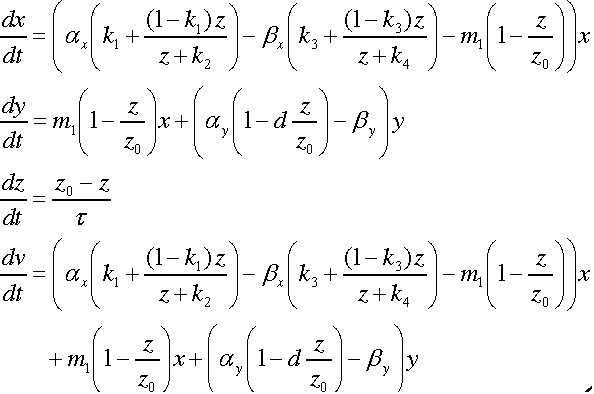
\includegraphics[width=0.45\textwidth]{images/prostatebw-mode2.pdf}
  }
  \hfill
  \subfloat[Visualization of a generated counterexample. Change in the shade of colors represents discrete mode changes.]{%
    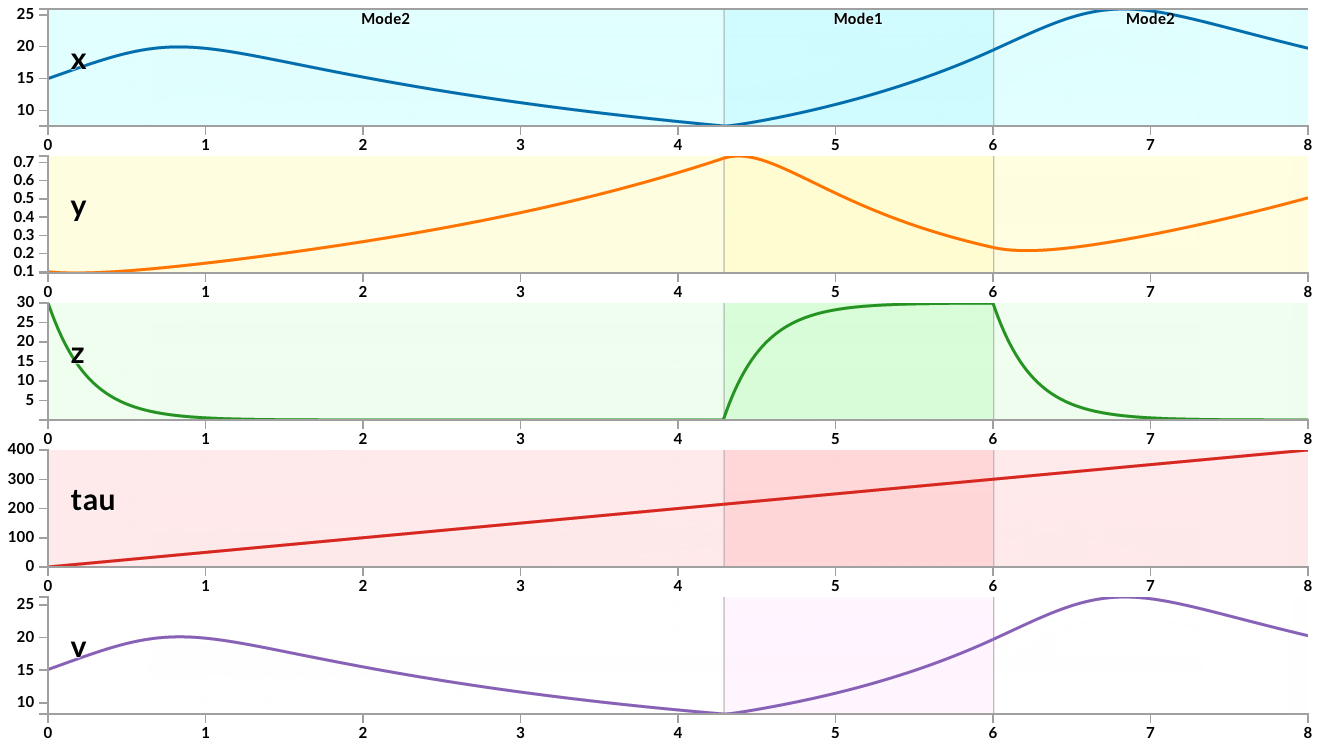
\includegraphics[width=0.48\textwidth]{images/prostate}
  }
  \caption{An example of nonlinear dynamics and counterexample-generation.}
  \label{fig:prostate-example}
\end{figure}

It is well-known that the standard bounded reachability problems for
simple hybrid systems are already highly
undecidable~\cite{DBLP:conf/hybrid/AlurCHH92}.
Instead, we work in the framework of $\delta$-reachability of hybrid systems~\cite{DBLP:journals/corr/GaoKCC14}.
Here $\delta$ is an arbitrary positive rational number, provided by the user to
specify the bound on numerical errors that can be tolerated in the analysis.
For a hybrid system $H$ and an unsafe region $\unsafe$ (both encoded as logic formulas),
the $\delta$-reachability problem asks for one of the following answers:
\begin{itemize}
        \item {\sf safe}: $H$ cannot reach $\unsafe$.
        \item {\sf $\delta$-unsafe}: $H^{\delta}$ can reach $\unsafe^{\delta}$.
\end{itemize}
Here, $H^{\delta}$ and $\unsafe^{\delta}$ encode ($\delta$-bounded) overapproximations
of $H$ and $\unsafe$, defined explicitly as their syntactic variants.%(See Section~\ref{sec:delta-reachability} in the Appendix.)
It is important to note that the definition makes the answers no weaker than standard reachability:
When {\sf safe} is the answer, we know for certain that $H$ does not reach
the unsafe region (no $\delta$ is involved); when {\sf $\delta$-unsafe} is the answer,
we know that there exists some $\delta$-bounded perturbation of the system that can render it unsafe.
Since $\delta$ can be chosen to be very small, {\sf$\delta$-unsafe} answers in fact
discover robustness problem in the system, which should be regarded as unsafe indeed.
We have proved that bounded $\delta$-reachabilty is decidable for a wide range
of nonlinear hybrid systems, even with reasonable complexity bounds~\cite{DBLP:journals/corr/GaoKCC14}.
This framework provides the formal correctness guarantees of \dReach{}.

Apart from solving $\delta$-reachability, the following key features of \dReach{}
distinguish it from other existing tools in this
domain~\cite{DBLP:journals/jlp/FranzleTE10,DBLP:conf/cav/FrehseGDCRLRGDM11,DBLP:journals/tac/AlthoffK14,DBLP:conf/hybrid/Frehse05,DBLP:conf/icons/HerdeEFT08,DBLP:conf/rtss/ChenAS12,DBLP:conf/aaai/CimattiMT12}.
%insert explanations for each item.
\begin{enumerate}
\item Expressiveness. \dReach{} allows the user to describe hybrid
  systems using first-order logic formulas over real numbers with a
  wide range of nonlinear functions. This allows the user to specify
  the continuous flows using highly nonlinear differential equations,
  and the jump and reset conditions with complex Boolean combinations
  of nonlinear constraints. \dReach{} also faithfully translates mode
  invariants into $\exists\forall$ logic formulas, which can be
  directly solved under certain restrictions on the invariants.
\item Property-guided search. \dReach{} maintains logical encodings
  (the same approach as~\cite{DBLP:conf/aaai/CimattiMT12}), whose size
  is linear in the size of the inputs, of the reachable states of a
  hybrid system~\cite{DBLP:journals/corr/GaoKCC14}. The tool searches
  for concrete counterexamples to falsify the reachability properties,
  instead of overapproximating the full reachable states. This avoids
  the usual state explosion problem in reachable set computation,
  because the full set of states does not need to be explicitly
  stored. This change is analogous to the difference between SAT-based
  model checking and BDD-based symbolic model checking.
\item Tight integration of symbolic reasoning and numerical solving.
  \dReach{} delegates the reasoning on discrete mode changes to SAT
  solvers, and uses numerical constraint solving to handle nonlinear
  dynamics. As a result, it can combine the full power of both
  symbolic reasoning and numerical analysis algorithms. In particular,
  all existing tools for reachable set computation can be easily
  plugged-in as engines for solving the continuous part of the
  dynamics, while logic reasoning tools can overcome the difficulty in
  handling complex mode transitions.
\end{enumerate}
The paper is structured as follows. We describe the system architecture in Section 2,
and give some details about the logical encoding in the tool in Section 3.
We then explain the input format and usage in Section 4. %More details and examples are given in the Appendix.

%Realistic hybrid systems involves nonlinear ODEs with transcendental
%functions. \dReach{} allows users to specify a hybrid system in a
%nonlinear signature as it is without linearizing or overapproximating
%it. Users can provide the tool with a numerical error bound $\delta$,
%a bounded time horizon $[0, T]$, and a maximum number of mode switches
%$k$ for the analysis. As a result of analysis, \dReach{} will return
%either \textbf{$\delta$-sat} with a concrete counterexample, or
%\textbf{unsat} which does not involve numerical errors. We also
%provide a visualization for the $\delta$-sat case to help
%understand the analysis result.

% TODO: Need to differentiate this paper from FMCAD paper
%  - FMCAD: underlying solving techniques for SMT with ODEs
%  - TACAS: tool, encoding, using solver...

%%% Local Variables:
%%% mode: latex
%%% TeX-master: "main"
%%% End:

%\section{Probabilistic bounded reachability for hybrid systems with parametric uncertainty}
\section{Probabilistic bounded reachability}

\hide{
\subsection{Hybrid automata with parametric uncertainty}
We present a model for hybrid systems with probabilistic parameters using the framework of hybrid automata \cite{henzinger2000theory}. A hybrid automaton with parametric uncertainty introduces a finite number of random 
parameters with given distributions.
\begin{definition}
\label{def:ha}
{\rm(Hybrid Automata with Parametric Uncertainty)} A hybrid automaton with probabilistic parameters $H_p$ consists of the following components.

{\bf Variables}. A finite set $X = \{ x_1, \cdots, x_n \}$ of real-numbered variables, where $n$ is the dimension of $H_p$. We write $\dot{X}$ for the set $\{\dot{x_1}, \cdots, \dot{x_n}\}$ to represent first derivatives of variables during the continuous change, and write $X'$ for the set $\{x_1', \cdots, x_n'\}$ to denote values of variables at the conclusion of the discrete change.

{\bf Random Variables}. A finite set $Y = \{ y_1, \cdots, y_m \}$ of discrete and continuous random variables, and the corresponding distribution set $Distr=\{distr_1, \cdots,\\ distr_m\}$, where, for $0 \le i \le m$, $y_i$ has the corresponding distribution $distr_i$. These random variables are used to describe the system uncertainty caused by probabilistic parameters.

{\bf Control graph}. A finite directed multigraph $(V,E)$. The vertices in $V$ are called control modes, and edges in $E$ are control switches.

{\bf Initial, invariant, and flow conditions}. As vertex labeling functions over each control mode $v \in V$, the initial condition $init(v)$ is predicate whose free variables are from $V$, the invariant condition $inv(v)$ is a predicate whose free variables are from $X$, and the flow condition $flow(v)$ is a predicate whose free variables are from $X \cup \dot{X}$.

{\bf Jump conditions}. An edge labeling function $jump$ that assigns to each control switch $e \in E$ a predicate whose free variables are from $X \cup X'$.

{\bf Events}. A finite set $\Sigma$ of events, and an edge labeling function $event: E \to \Sigma$ that assigns to each control switch an event. 
 
\end{definition}

\subsection{Probabilistic bounded reachability}
With respect to system analysis, we are interested in the probability of reaching the target states within a bounded number of transition steps. We now formally state the probabilistic reachability problem for hybrid automata with parametric uncertainty. 

Let $H$ be a hybrid automaton without parametric uncertainty, and $H_p$ be a system of hybrid automata with parametric uncertainty as in Definition \ref{def:ha}. As for the set of random variables $Y_{H_p}$, let $\Omega_{H_p}$ be the corresponding sample space. we write $S$ as a random sampler with respect to the joint distribution of all random variables - $S: Y_{H_p} \to \omega_{H_p}$. For each sample $s_i$ generated by $S$, we write $H_{p}[s_i/Y_{H_p}]$ as the corresponding hybrid automaton without parametric uncertainty, where the set of random variables $Y_{H_p}$ has been replaced by their corresponding sampled values in $s_i$. Let $k \in N$ be a step bound, and $R_{H}^k$ denotes the set of all initialized trajectories of length $k$ of $H$. Also, we write $Goal$ be the set of target states.
\begin{remark}
\label{def:br}
{\rm (Bounded Reachability for Hybrid Automata)}
The bounded reachability problem for $H$ asks if there is a trace $\sigma \in R_{H}^k$ that visits the $Goal$.
\end{remark}
\begin{definition}
\label{def:pbr}
{\rm (Probabilistic Bounded Reachability for Hybrid Automata with Parametric Uncertainty)}\\
The probabilistic bounded reachability for $H_p$ estimates the maximum probability, over $\Omega_{H_p}$, of the bounded reachability for $H_{p}[s_i/Y_{H_p}]$, where $s_i \in S(Y_{H_p})$.
\end{definition}
}

To solve the probabilistic bounded reachability problem for a given hybrid model with probabilistic parameters $MP$, our method first samples the involved set of random variables, denoted as $RV$, according to their distributions. Then, according to each sample $S_i$, we obtain a model of the hybrid system without any probabilistic parameters $M_i$. {\bf SReach} then calls {\bf dReach} \cite{gaodelta} with the precision $\delta$ and the unfolding steps $k$. {\bf dReach} is a bounded reachability analyzer based on {\bf dReal} \cite{gao2013dreal}, and returns either unsat or $\delta$-sat for $M_i$. With a sufficient number of sampled models, and a specified statistical testing method $ST$, {\bf SReach} terminates the entire procedure. It either returns the maximal probability of the system satisfying the given reachability property, or accepts or rejects according to the comparison whether the returned probability is larger (or smaller) than the specified threshold. Algorithm \ref{fig:sreach} illustrates the main algorithm of our approach.
\begin{algorithm}
  \centering
  \caption{SReach}
  \label{fig:sreach}
  \begin{algorithmic}[1]
    \Function{SReach}{$MP$, $ST$, $\delta$, $k$}
        \State $Succ \gets 0$	\Comment{number of $\delta$-sat samples}
        \State $N \gets 0$	\Comment{total number of samples}
        \State $RV \gets \mathrm{ExtractRV}(MP)$	\Comment{get the RVs from the probabilistic model}
        \Repeat
            \State $S_i \gets \mathrm{Sim}(RV)$		\Comment{sample the parameters}
            \State $M_i \gets \mathrm{Gen}(MP, S_i)$	\Comment{generate a dReach model}
            \State $Res \gets \mathrm{dReach}(M_i, \delta, k)$	\Comment{call dReach to solve $k$-step $\delta$-reachability}
            \If{$Res$ = $\delta$-sat}
            	%Good
		\State $Succ \gets Succ + 1$
%	  \Else
%	   	%Bad
%		\State $Fail \gets Fail + 1$
	    
	  \EndIf
	\State $N \gets N + 1$
        \Until{$ST.done(Succ, N)$}	\Comment{perform statistical test}\\
        %\State $Est\_prob \gets Succ / N$
	\quad\hspace{0.5ex} \Return $ST.output$
   \EndFunction
  \end{algorithmic}
\end{algorithm}

Consider a hybrid system $H$ with parametric uncertainty  and a reachability property $\phi$. {\bf SReach} 
can be used to answer two types of questions: (1) Qualitative: Does $H$ satisfy $\phi$ with probability
greater than a certain threshold? and (2) Quantitative: What is the probability that $H$ satisfies $\phi$?
Qualitative questions can be answered by hypothesis testing, while quantitative questions are addressed with
statistical estimation methods. Both methods produce answers up to some correctness 
precision that can be set arbitrarily by the user.
We have implemented in {\bf SReach} a number of statistical estimation and hypothesis testing techniques ---
more details can be found in Appendix \ref{apndx:stat}.

\section{Experiments}
\vspace{-.1cm}
Our method is implemented in the open-source tool {\bf SReach} (\url{https://github.com/rachelwang/SReach}). See Appendix \ref{apndx:usage} for its usage. All benchmarks and data shown below are on the tool website. All experiments were conducted on a machine with 2.9GHz Intel Core i7 processor and 8GB RAM, running OS X 10.9.2. 
In our experiments we used $0.001$ as the precision for the $\delta$-decision problem; and Bayesian sequential estimation
with $0.01$ half-interval width, coverage probability $0.99$, and uniform prior ($\alpha = \beta = 1$). The 
detailed description of the following models in Appendix \ref{apndx:model} demonstrates their highly nonlinear and nondeterministic characteristics.

{\bf\noindent Prostate cancer treatment.}
%\textit{Model Description}.
We modified the model of the intermittent androgen suppression (IAS) therapy in \cite{tanaka2010mathematical} by adding parametric uncertainty. The IAS therapy switches between  treatment-on, and treatment-off with respect to the serum level thresholds of prostate-specific antigen (PSA) - $r_0$ and $r_1$. As suggested by the clinical trials \cite{bruchovsky2006final}, an effective IAS therapy highly depends on the individual patient. Thus, we modified the model by taking the parametric variation caused by the personalized differences into account. In details, according to the clinic data from hundreds of patients \cite{bruchovsky2007locally}, we replaced 6 system 
parameters with random variables with appropriate (continuous) distributions, including $\alpha_x$ (proliferation rate of AD cells), $\alpha_y$ (proliferation rate of AI cells), $\beta_x$ (apoptosis rate of AD cells), $\beta_y$ (apoptosis rate of AI cells), $m_1$ (mutation rate from AD to AI cells), and $z_0$ (normal androgen level).
\vspace{-.5cm}
\begin{table}[th!]
\captionsetup{font=scriptsize}
\centering
    \begin{tabular}{c|c|c|c|c|c|c|c|c}
    \hline
    Model & \#RVs & $r_0$ & $r_1$ & Est\_P & \#S\_S & \#T\_S & Avg\_T(s) & Tot\_T(s) \\ \hline
    PCT1  & 6     & 5.0  & 10.0 & 0.04   & 0      & 227    & 0.145   & 32.915     \\ \hline
    PCT2  & 6     & 7.0  & 11.0 & 0.591  & 2144   & 3628   & 432.491 & 1569077.348     \\ \hline
    PCT3  & 6     & 10.0 & 15.0 & 0.996  & 227    & 227    & 692.861   & 157279.446   \\ \hline
    \end{tabular}
    \caption{\#RVs = number of random variables in the model, \#S\_S = number of $\delta$-sat samples, 
\#T\_S = total number of samples, $r_0$ = lower threshold of the serum PSA level, $r_1$ = upper threshold, 
Est\_P = estimated probability of the property,  Avg\_T(s) = average CPU time of each sample in seconds, and Tot\_T(s) = total CPU time for all samples in seconds.}
    \label{table:prostate}
\end{table}
\vspace{-1.1cm}
%\subsection{Cardiac models}
%\textit{Experiments and Results} 

To describe the variations due to individual difference, we assigned $\alpha_x$ to be $U(0.0193, 0.0214)$, $\alpha_y$ to be $U(0.0230, 0.0254)$, $\beta_x$ to be $U(0.0072, 0.0079)$, $\beta_y$ to be $U(0.0160, 0.0176)$, $m_1$ to be $U(0.0000475, 0.0000525) $, and $z_0$ to be $N(30.0, 0.001)$. 
We used {\bf SReach} to estimate the probabilities of the model preventing the relapse of the prostate cancer with three distinct pairs of treatment thresholds (\ie, combinations of $r_0$ and $r_1$).  In the experiments, we chose 2 as the unfolding steps. For each sample generated, {\bf SReach} dealt with $41$ variables, and $10$ ODEs. As shown in Table \ref{table:prostate}, the model with thresholds $r_0 = 10$, and $r_1 = 15$ has the probability approaching to 1, indicating that these thresholds can be considered for the general treatment. 

{\bf\noindent Atrial Fribrillation.} The minimum resistor model (MRM) reproduces experimentally measured characteristics 
of human ventricular cell dynamics \cite{bueno2008minimal}. 
The MRM reduces the complexity of existing models by representing channel gates of different ions with one fast channel, and two slow gates. However, due to this reduction, for most model parameters, it becomes impossible to obtain their values through measurements. With this application, we will show that {\bf SReach} can also be adopted to identify appropriate ranges and distributions for model parameters, \ie, parameter estimation.

%\textit{Experiments and Results} 
To illustrate the way that {\bf SReach} is used to conduct parameter estimation, we chose two system parameters - $EPI\_TO1$, and $EPI\_TO2$, and varied their distributions to see with which distributions for these two system parameters, the model can present the desired pattern. The model has 4 modes. In the experiments, we chose $3$ as the unfolding steps. For each sample generated, {\bf SReach} dealt with $62$ variables, and $24$ ODEs. As in the Table \ref{table:cardiac}, when $EPI\_TO1$ is either close to $400$, or between $0.0061$ and $0.007$, and $EPI\_TO2$ is close to $6$, the model can satisfy the given bounded reachability property with a probability very close to $1$. 
\vspace{-.5cm}
\begin{table}[h!]
\captionsetup{font=scriptsize}
\centering
    \begin{tabular}{c|c|c|c|c|c|c|c|c}
    \hline
    Model         & \#RVs & EPI\_TO1            & EPI\_TO2         & \#S\_S & \#T\_S & Est\_P &  A\_T(s) & T\_T(s) \\ \hline
    Cd\_to1\_s    & 1     & U(6.1e-3, 7e-3)    & 6              & 227       & 227      & 0.996     & 0.362   & 82.174     \\ \hline
    Cd\_to1\_uns  & 1     & U(5.5e-3, 5.9e-3)   & 6              & 0         & 227      & 0.004     & 0.124 & 28.148       \\ \hline
    Cd\_to2\_s    & 1     & 400               & U(0.131, 6)    & 227       & 227      & 0.996     & 0.361  & 81.947      \\ \hline
    Cd\_to2\_uns  & 1     & 400               & U(0.1, 0.129)    & 0         & 227      & 0.004     & 0.139   & 31.552     \\ \hline
    Cd\_to12\_s   & 2     & N(400, 1e-4)      & N(6, 1e-4)     & 227       & 227      & 0.996     & 0.373  & 84.671      \\ \hline
    Cd\_to12\_uns & 2     & N(5.5e-3, 10e-6) & N(0.11, 10e-5) & 0         & 227      & 0.004     & 0.131  & 29.737      \\ \hline
    \end{tabular}
    \caption { \#RVs = number of random variables in the model, \#S\_S = number of $\delta$-sat samples, 
\#T\_S = total number of samples, Est\_P = estimated probability of property,  A\_T(s) = average 
CPU time of each sample in seconds, and T\_T(s) = total CPU time for all samples in seconds.}
    \label{table:cardiac}
\end{table}
\vspace{-1cm}

\begin{comment}

\subsection{Application to the stabilization control of quadcopters}

\textit{Model Description}.
We modeled the stabilization control of a quadcopter, and are interested in analyzing its robustness. In other words, given an arbitrary initial location and position, this model will guarantee that the quadcopter will soon become stable via adjusting velocities of four rotors. To specify the arbitrary initial status, we introduced 6 random variables: ($x_0$, $y_0$, $z_0$) (the initial location),  $\phi_0$ (the initial roll angle), $\theta_0$ (the initial pitch angle), and $\psi_0$ (the initial yaw angle).

\textit{Experiments and Results}. To validate this model, {\bf SReach} was adopted with the BIFT statistical testing option.  

\end{comment}

{\noindent\bf Additional benchmarks.} To further demonstrate the feasibility of {\bf SReach}, we also applied it to the following benchmarks. 
Table \ref{table:exp} shows the results of experiments. BB refers to the bouncing ball models, 
Tld the thermostat model with linear temperature decrease, Ted the thermostat model with exponential decrease, 
DT the dual thermostat models, W the watertank models, DW the dual watertank models, 
%Gear the gear shift control model, 
Que the model for queuing system, 3dOsc the model for 3d oscillator, and QuadC the model for quadcopter 
stabilization control. 
\vspace{-.5cm}
\begin{table}[h!]
\captionsetup{font=scriptsize}
\centering
    \begin{tabular}{c|c|c|c|c|c|c|c|c|c|c|c}
    \hline
    Benchmark & \#Ms & K & \#ODEs & \#Vs & \#RVs & $\delta$ & Est\_P & \#S\_S & \#T\_S &  A\_T(s) & T\_T(s)  \\ \hline
    BBK1      & 1       & 1 & 2      & 14    & 3     & 0.001 & 0.754  & 5372      & 7126     & 0.086  & 612.836         \\ \hline
    BBK5      & 1       & 5 & 2      & 38    & 3     & 0.001 & 0.059  & 209       & 3628     & 0.253   &  917.884       \\ \hline
    BBwDv1    & 2       & 2 & 4      & 20    & 4     & 0.001 & 0.208  & 2206      & 10919    & 0.080   &  873.522     \\ \hline
    BBwDv2K2  & 2       & 2 & 4      & 20    & 3     & 0.001 & 0.845  & 7330      & 8669     & 0.209    & 1811.821      \\ \hline
    BBwDv2K8  & 2       & 8 & 4      & 56    & 3     & 0.001 & 0.207  & 2259      & 10901    & 0.858  & 9353.058        \\ \hline
    Tld       & 2       & 7 & 2      & 33     & 4     & 0.001 & 0.996      & 227         & 227        & 0.213     & 48.351         \\ \hline
    Ted       & 2       & 7 & 4      & 50     & 4     & 0.001 & 0.996      & 227         & 227       & 12.839   & 2914.448     \\ \hline
    DTldK3    & 2       & 3 & 4      & 26    & 2     & 0.001 & 0.996  & 227       & 227      & 0.382    & 86.714      \\ \hline
    DTldK5    & 2       & 5 & 4      & 38    & 2     & 0.001 & 0.161  & 1442      & 8961     & 0.280  &  2509.078       \\ \hline
    W4mv1       & 4       & 3 & 8      & 26     & 6     & 0.001 & 0.381      & 5953         & 15639        & 0.238   & 3722.082     \\ \hline
    W4mv2K3       & 4       & 3 & 8      & 26     & 6     & 0.001 & 0.996      & 227         & 227        & 0.673   & 152.771      \\ \hline
    W4mv2K7       & 4       & 7 & 8      & 50     & 6     & 0.001 & 0.004     & 0         & 227        & 0.120    & 27.240          \\ \hline
    DWK1      & 2       & 1 & 4      & 14    & 5     & 0.001 & 0.996  & 227       & 227      & 0.171   & 38.817      \\ \hline
    DWK3      & 2       & 3 & 4      & 26    & 5     & 0.001 & 0.996  & 227       & 227      & 0.215    & 48.806      \\ \hline
    DWK9      & 2       & 9 & 4      & 62    & 5     & 0.001 & 0.996  & 227       & 227      & 5.144   &  1167.688      \\ \hline
   % Gear      & 4       & ~ & ~      & ~     & ~     & 0.001 & ~      & ~         & ~        & ~     & ~          \\ \hline
    Que       & 3       & 2 & 3      & 13     & ~     & 0.001 & 0.228      & 2662         & 11677        & 0.095   & 1109.315   \\ \hline
    3dOsc     & 3       & 2 & 18      & 48     & 2     & 0.001 & 0.996      & 227         & 227        & 8.273  & 1877.969   \\ \hline
    QuadC     & 1       & 0 & 14      & 44     & 6     & 0.001 & 0.996      & 227         & 227        & 825.641 & 187420.507   \\ \hline
    \end{tabular}
    \caption {\#Ms = number of modes, K indicates the unfolding steps, \#ODEs = number of ODEs in the model, \#Vs = number of total variables in the unfolded formulae, \#RVs = number of random variables in the model, $\delta$ = precision used in 
{\bf dReach}, \#S\_S = number of $\delta$-sat samples , \#T\_S = total number of samples, Est\_P = estimated 
probability of the property,  A\_T(s) = average CPU time of each sample in seconds, and T\_T(s) = total CPU time for all samples in seconds.}
    \label{table:exp}
\end{table}
\vspace{-1.1cm}

\section{Conclusion and future work}
In conclusion, we presented a reachability analysis tool. The tool combines $\delta$-decision procedure \cite{gao2013dreal, gao2013satisfiability, gaodelta} and statistical testing techniques. It supports bounded reachability analysis and parameter estimation for hybrid systems with parametric uncertainty. This tool was used for the reachability analysis of two representative examples - the prostate cancer treatment control and the cardiac system, and of additional 19 benchmarks. In the near future, we plan to support the reachability analysis for more general stochastic hybrid models, where, besides probabilistic system parameters, there also exist probabilistic jumps with discrete or continuous distributions. 


\bibliography{ref}{}
\bibliographystyle{abbrv}

\newpage
\appendix
\hide{
\newpage
\section*{Appendix: $\lrf$-Formulas and $\delta$-Decidability}

We will use a logical language over the real numbers that allows arbitrary {\em computable real functions}~\cite{CAbook}. We write $\lrf$ to represent this language. Intuitively, a real function is computable if it can be numerically simulated up to an arbitrary precision. For the purpose of this paper, it suffices to know that almost all the functions that are needed in describing hybrid systems are Type 2 computable, such as polynomials, exponentiation, logarithm, trigonometric functions, and solution functions of Lipschitz-continuous ordinary differential equations.

More formally, $\lrf = \langle \mathcal{F}, > \rangle$ represents the first-order signature over the reals with the set $\mathcal{F}$ of computable real functions, which contains all the functions mentioned above. Note that constants are included as 0-ary functions. $\lrf$-formulas are evaluated in the standard way over the structure $\mathbb{R}_{\mathcal{F}}= \langle \mathbb{R}, \mathcal{F}^{\mathbb{R}}, >^{\mathbb{R}}\rangle$. It is not hard to see that  we can put any $\lrf$-formula in a normal form, such that its atomic formulas are of the form $t(x_1,...,x_n)>0$ or $t(x_1,...,x_n)\geq 0$, with $t(x_1,...,x_n)$ composed of functions in $\mathcal{F}$. To avoid extra preprocessing of formulas, we can explicitly define $\mathcal{L}_{\mathcal{F}}$-formulas as follows.
\begin{definition}[$\lrf$-Formulas]
Let $\mathcal{F}$ be a collection of computable real functions. We define:
\begin{align*}
t& := x \; | \; f(t(\vec x)), \mbox{ where }f\in \mathcal{F} \mbox{ (constants are 0-ary functions)};\\
\varphi& := t(\vec x)> 0 \; | \; t(\vec x)\geq 0 \; | \; \varphi\wedge\varphi
\; | \; \varphi\vee\varphi \; | \; \exists x_i\varphi \; |\; \forall x_i\varphi.
\end{align*}
In this setting $\neg\varphi$ is regarded as an inductively defined operation
which replaces atomic formulas $t>0$ with $-t\geq 0$, atomic formulas $t\geq 0$
with $-t>0$, switches $\wedge$ and $\vee$, and switches $\forall$ and $\exists$.
\end{definition}
\begin{definition}[Bounded $\lrf$-Sentences]
We define the bounded quantifiers $\exists^{[u,v]}$ and $\forall^{[u,v]}$ as
$\exists^{[u,v]}x.\varphi =_{df}\exists x. ( u \leq x \land x \leq v \wedge
\varphi)$ and $
\forall^{[u,v]}x.\varphi =_{df} \forall x. ( (u \leq x \land x \leq v)
\rightarrow \varphi)$
where $u$ and $v$ denote $\lrf$ terms, whose variables only
contain free variables in $\varphi$ excluding $x$. A {\em bounded $\lrf$-sentence} is
$$Q_1^{[u_1,v_1]}x_1\cdots Q_n^{[u_n,v_n]}x_n\;\psi(x_1,...,x_n),$$
where $Q_i^{[u_i,v_i]}$ are bounded quantifiers, and $\psi(x_1,...,x_n)$ is
quantifier-free.
\end{definition}
\begin{definition}[$\delta$-Variants]\label{variants}
Let $\delta\in \mathbb{Q}^+\cup\{0\}$, and $\varphi$ an
$\lrf$-formula
$$\varphi: \ Q_1^{I_1}x_1\cdots Q_n^{I_n}x_n\;\psi[t_i(\vec x, \vec y)>0;
t_j(\vec x, \vec
y)\geq 0],$$ where $i\in\{1,...k\}$ and $j\in\{k+1,...,m\}$. The {\em
$\delta$-weakening} $\varphi^{\delta}$ of $\varphi$ is
defined as the result of replacing each atom $t_i > 0$ by $t_i >
-\delta$ and $t_j \geq 0$ by $t_j \geq -\delta$:
$$\varphi^{\delta}:\ Q_1^{I_1}x_1\cdots Q_n^{I_n}x_n\;\psi[t_i(\vec x, \vec
y)>-\delta; t_j(\vec x,
\vec y)\geq -\delta].$$
It is clear that $\varphi\rightarrow\varphi^{\delta}$~(see \cite{gao12b}).
\end{definition}
In~\cite{dreal}, we have proved that the following $\delta$-decision problem is decidable, which is the basis of our framework.
\begin{theorem}[$\delta$-Decidability]\label{delta-decide} Let $\delta\in\mathbb{Q}^+$ be
arbitrary. There is an algorithm which, given any bounded $\lrf$-sentence $\varphi$,
correctly returns one of the following two answers:
\begin{itemize}
\item $\delta$-$\mathsf{True}$: $\varphi^{\delta}$ is true.
\item $\mathsf{False}$: $\varphi$ is false.
\end{itemize}
When the two cases overlap, either answer is correct.
\end{theorem}
\begin{theorem}[Complexity]\label{compmain}
Let $S$ be a class of $\lrf$-sentences, such that for any $\varphi$ in $S$, the terms in $\varphi$ are in Type 2 complexity class $\mathsf{C}$. Then, for any $\delta\in \mathbb{Q}^+$, the $\delta$-decision problem for bounded $\Sigma_n$-sentences in $S$ is in $\mathsf{(\Sigma_n^P)^C}$.
\end{theorem}


\section*{Appendix: BCF Model in dReach}

\begin{verbatim}
//Translated to drh by Sicun Gao on Apr-18-2013
// ===============================================================
// ==   Minimal Resistor Model (4 state variables)              ==
// ==                                                           ==
// ==   Author:  E. Bartocci                                    ==
// ==                                                           ==
// ==   Date:  11/05/10                                         ==
// ==                                                           ==
// ==   Free distribution with authors permission               ==
// ==                                                           ==
// ==   SUNY Stony Brook, Stony Brook, NY                       ==
// ==                                                           ==
// ===============================================================
// The following are the parameters that you can find in the paper
// A. Bueno-Orovio, M. Cherry, and F. Fenton, `Minimal model for
// human ventricular action potentials in tissue', Journal of
// Theoretical Biology, no. 253, pp. 544?560, 2008.
// ===============================================================

#define  EPI_TVP         1.4506
#define  EPI_TV1M       60.0
#define  EPI_TV2M     1150.0
#define  EPI_TWP       200.0
#define  EPI_TW1M       60.0
#define  EPI_TW2M       15.0

#define  EPI_TS1        2.7342
#define  EPI_TS2       16.0     //The same with Flavio's paper
#define  EPI_TFI        0.11    //The same with Flavio's paper

#define  EPI_TO1      400    //The same with Flavio's paper
#define  EPI_TO2        6.0      //The same with Flavio's paper
#define  EPI_TSO1      30.0181 //The same with Flavio's paper
#define  EPI_TSO2       0.9957  //The same with Flavio's paper

#define  EPI_TSI        1.8875  // We have TSI1 and TSI2 TSI in Flavio's paper


#define  EPI_TWINF      0.07    //The same with Flavio's paper
#define  EPI_THV        0.3     //EPUM The same of Flavio's paper
#define  EPI_THVM       0.006   //EPUQ The same of Flavio's paper
#define  EPI_THVINF     0.006   //EPUQ The same of Flavio's paper
#define  EPI_THW        0.13    //EPUP The same of Flavio's paper
#define  EPI_THWINF     0.006   //EPURR In Flavio's paper 0.13
#define  EPI_THSO       0.13    //EPUP The same of Flavio's paper
#define  EPI_THSI       0.13    //EPUP The same of Flavio's paper
#define  EPI_THO        0.006   //EPURR The same of Flavio's paper

#define  EPI_KWM       65.0     //The same of Flavio's paper
#define  EPI_KS         2.0994  //The same of Flavio's paper
#define  EPI_KSO        2.0458  //The same of Flavio's paper

#define  EPI_UWM        0.03    //The same of Flavio's paper
#define  EPI_US         0.9087  //The same of Flavio's paper
#define  EPI_UO         0.0     //The same of Flavio's paper
#define  EPI_UU         1.55    //The same of Flavio's paper
#define  EPI_USO        0.65    //The same of Flavio's paper

#define  jfi1  0.0
#define  jso1  (u/EPI_TO1)
#define  jsi1  0.0

#define  jfi2  0.0
#define  jso2  (u/EPI_TO2)
#define  jsi2  0.0


#define  jfi3  0.0
#define  jso3  1.0/(EPI_TSO1+((EPI_TSO2- EPI_TSO1)*(1/(1+exp(-2*EPI_KSO*(u- EPI_USO))))))
#define  jsi3  (0 - (w * s)/EPI_TSI)

#define  jfi4  (0 - v * (u - EPI_THV) * (EPI_UU - u)/EPI_TFI)
#define  jso4  (1.0 / (EPI_TSO1+((EPI_TSO2 - EPI_TSO1)*(1/(1+exp(-2*EPI_KSO*(u- EPI_USO)))))))
#define  jsi4  ( 0 - (w * s)/EPI_TSI)
#define	 stim  1.0 // The external stimulation is a rectangular pulse of 
                      height 1 and length 1ms. Since u reach its maximum 
                      during the stimulation, time scale is set to be [0,1] 
[0, 2.0] u;
[0, 2.0] v;
[0, 2.0] w;
[0, 2.0] s;
[0, 1] tau;
[0, 1] time;

{mode 1;

invt:    (u >= 0);
         (u <= 0.006);
         (v >= 0);
         (w >= 0);
         (s >= 0);
         (tau >= 0);
flow:
         d/dt[tau] = 1.0;
         d/dt[u] = (stim - jfi1) - (jso1 + jsi1);
         d/dt[w] = ((1.0 -(u/EPI_TWINF) - w)/(EPI_TW1M + (EPI_TW2M - EPI_TW1M) * 
                   (1/(1+exp(-2*EPI_KWM*(u - EPI_UWM))))));
         d/dt[v] = ((1.0 - v)/EPI_TV1M);
         d/dt[s] = (((1/(1+exp( -2 * EPI_KS * (u - EPI_US) ))) - s)/EPI_TS1);
jump:
         (u >= 0.006) ==> @2 (and (tau' = tau) (u' = u) (v'= v) (w' = w) (s' = s));
}

{mode 2;

invt:
         (u >= 0.006);
         (u <= 0.13);
         (v >= 0);
         (w >= 0);
         (s >= 0);
         (tau >= 0);
flow:
         d/dt[tau] = 1.0;
         d/dt[u] = (stim - jfi2) - (jso2 + jsi2);
         d/dt[w] = ((0.94-w)/(EPI_TW1M + (EPI_TW2M - EPI_TW1M) * 
                   (1/(1+exp(-2*EPI_KWM*(u - EPI_UWM))))));
         d/dt[v] = (-v/EPI_TV2M);
         d/dt[s] = (((1/(1+exp( -2 * EPI_KS * (u - EPI_US) ))) - s)/EPI_TS1);
jump:
         (u >= 0.13) ==> @3 (and (tau' = tau) (u' = u) (v'= v) (w' = w) (s' = s));
}

{mode 3;

invt:
         (u >= 0.13);
         (u <= 0.3);
         (v >= 0);
         (w >= 0);
         (s >= 0);
         (tau >= 0);
flow:
         d/dt[tau] = 1.0;
         d/dt[u] = (stim - jfi3) - (jso3 + jsi3);
         d/dt[w] = (-w/EPI_TWP);
         d/dt[v] = (-v/EPI_TV2M);
         d/dt[s] = (((1/(1+exp( -2 * EPI_KS * (u - EPI_US) ))) - s)/EPI_TS2);
jump:
         ( u >= 0.3) ==> @4 (and (tau' = tau) (u' = u) (v'= v) (w' = w) (s' = s));
}

{mode 4;

invt:
         (u >= 0.3);
         (v >= 0);
         (w >= 0);
         (s >= 0);
         (tau >= 0);
flow:
         d/dt[tau] = 1.0;
         d/dt[u] =  (stim - jfi4) - (jso4 + jsi4);
         d/dt[w]  = (-w/EPI_TWP);
         d/dt[v]  = (-v/EPI_TVP);
         d/dt[s]  = (((1/(1+exp( -2 * EPI_KS * (u - EPI_US) ))) - s)/EPI_TS2) ;
jump:
         (u > 2.0) ==> @4 (and (tau' = tau) (u' = u) (v'= v) (w' = w) (s' = s));
}

init:  @1 (and (tau = 0) (u = 0.0) (v = 1.0) (w = 1.0) (s = 0.0));

goal:  @4 (and (tau = 1) (u >= 0.3) (u <= 2) (v >= 0) (v <= 2) 
          (w >= 0) (w <= 2) (s >= 0) (s <= 2));
\end{verbatim}


\section{The SReach tool}\label{apndx:usage}
\subsection{Input format}
The inputs to our {\bf SReach} tool are descriptions of hybrid automata with random variables (representing the probabilistic system parameters), and the reachability property to be checked. Following roughly the same format as the above definition of hybrid automata, and adding the declarations of random variables, the description of a automaton is of the following structure.

{\bf Preprocessor.} We can use the C language syntax to define constants and macros. When defining, random variables, which will be declared later, can also be used. 

\begin{comment}
For example, we can write,\\

$\#define\;\; x \;\;2.0$\\
$\#define\;\; y\;\; (z^2 \;+\; 1)$\\

where $z$ can be a random variable.\\
\end{comment}

{\bf Variable declaration.} For a random variable, the declaration specifies its distribution and name. For the variables which are not random variables, they are required to be declared within bounds. 
\begin{comment}
with the format - $Dist \; \; var_nam;$, where currently "$Dist$" can be "$B(p)$" (Bernoulli distribution), "$U(p, \;q)$" (Uniform distribution), "$N(p, \;q)$" (Gaussian distribution), and "$E(p)$" (Exponential distribution). $p$ and $q$ are parameters for these distributions. (Note: it is easy to include additional distributions if needed.)

For instance,\\
$[-10, \; 20.1]\; \;  x;$\\
\end{comment}

{\bf Hybrid automaton.} A hybrid automaton is represented by a set of modes. Within each mode declaration, users can specify statements for mode invariant(s), flow function(s), and jump condition(s). For a mode invariant, we can give any logic formula for the variables. For a flow function, it is expressed by an ODE.  As for a jump condition, it is written as 
\begin{verbatim} 
<logic_formula1>  ==> @<tagert_mode>  <logic_formula2>,
\end{verbatim}
where the first logic formula is given as the guard of the jump, and the later one specifies the reset condition after the jump.

\begin{comment}
each differential equation is of the format: "$d/dt \; [<var>]\;\;=\;\;<fun>;$". 

$
\{\;\; mode \;\; <int>;\\
invt: \;\; <mode\_invariant\; block>\\
flow: \;\; <ODE\; block>\\
jump: \;\; <jump\;block>\\
\}
$\\
\end{comment}


{\bf Initial conditions and Goals.} Following the declaration of modes, we can declare one initial mode with corresponding conditions, and the reachability properties in the end.\\
\begin{comment}
 via the following structure.\\

$
@Mode\_num\;\;\; [initial\_conditions]
$\\

{\bf Goals.} We can add the reachability properties in the end. Each property can be encoded in the following format.\\

$
@Mode\_num \;\;\; [reachability\_property]
$\\

\end{comment}

\noindent\textit{Example 3.1}. The following is an example input file. Currently, users can specify random variables with Bernoulli distribution, Uniform distribution, Gaussian distribution, and Exponential distribution. (Note: it is easy to include additional distributions if needed.)
\lstset{basicstyle=\ttfamily\small, numbers=left, breaklines=true }
\begin{lstlisting}
#define pi 3.1416
N(1,0.1) mu1;
U(10,15) thro;
E(0.49) theta1;
B(0.75) xinit;
[0,5] x;
[0,3] time;
{ mode 1; 
  invt:
         (x<=1.5);
         (x>=0);
  flow:
	 d/dt[x]=thro*(1/(theta1*sqrt(2*pi)))
	          *exp(0-((x-mu1)^2)/(2*theta1^2));
  jump:
        (x>=(thre1+5))==>@2(x'=x);
}
init:
@1	(x=xinit);
goal:
@4	(x>=50);
\end{lstlisting}

\subsection{Command line}
After building, {\bf SReach} can be simply used through:
\begin{verbatim} 
SReach <statistical_testing_option> <filename> <dReach> <k> <delta>
\end{verbatim} 
where:
\begin{itemize}
\item \verb+statistical_testing_option+ is a text file containing a sequence of test specifications. We will introduce the usages of statistical testing options in the following part;
\item \verb+filename+ is a .pdrh file describing the model of a hybrid system with probabilistic system parameters. It is of the input format described in last sub-section;
\item \verb+dReach+ is a bounded reachability analyzing tool for hybrid systems based on dReal;
\item \verb+k+ is the number of steps of the model that the tool will explore; and
\item \verb+delta+ is the precision for the $\delta$-decision problem.
\end{itemize}

\subsection{Statistical testing options}

{\bf SReach} can be used with different statistical testing methods through the following specifications.

\textit {Lai's test}: \verb+Lai <theta> <cost_per_sample>+, where \verb+theta+ indicates the probability threshold.
 
\textit {Bayes factor test}: \verb+BFT <theta> <T> <alpha> <beta>+,
where \verb+theta+ is a probability threshold satisfying \verb+0 < theta < 1+, \verb+T+ is a ratio threshold satisfying \verb+T > 1+, and \verb+alpha+, and \verb+beta+ are beta prior parameters.

\textit {BFT with indifference region}: \verb+BFTI <theta> <T> <alpha> <beta> <delta>+,
where, besides the parameters used in the above Bayes factor test, \verb+delta+ is given to create the indifference region - [$p_0$, $p_1$], where $p_0$ = \verb+theta+ + \verb+delta+ and $p_1$ = \verb+theta+  - \verb+delta+.  Now, it tests $H_0 :\; p \ge p_0$ against $H_1:\; p \le p_1$ .

\textit {Sequential probability ratio test (SPRT)}: \verb+SPRT <theta> <T> <delta>+.

\textit {Chernoff-Hoeffding bound}: \verb+CHB <delta1> <coverage_probability>+,
where \verb+delta1+ is the given precision, and \verb+coverage_probability+ indicates the confidence.

\textit {Bayesian Interval Estimation with Beta prior}: \\ \verb+BEST <delta1> <coverage_probability> <alpha> <beta>+.



}

\end{document}
